\section{Resultados}\label{sec:resultados}

Os valores desta seção estão em \texttt{metricas.csv}, gerado a partir dos registros pelo script \texttt{figuras\_lateral.py}.

\subsection{Referências geométricas}

A \autoref{fig:geo-trajetorias} mostra o caminho do eixo dianteiro a $1{,}0\,\mathrm{m/s}$ e a \autoref{tab:geo} resume as métricas. Todos os ensaios foram concluídos.

\begin{figure}[ht]
    \centering
    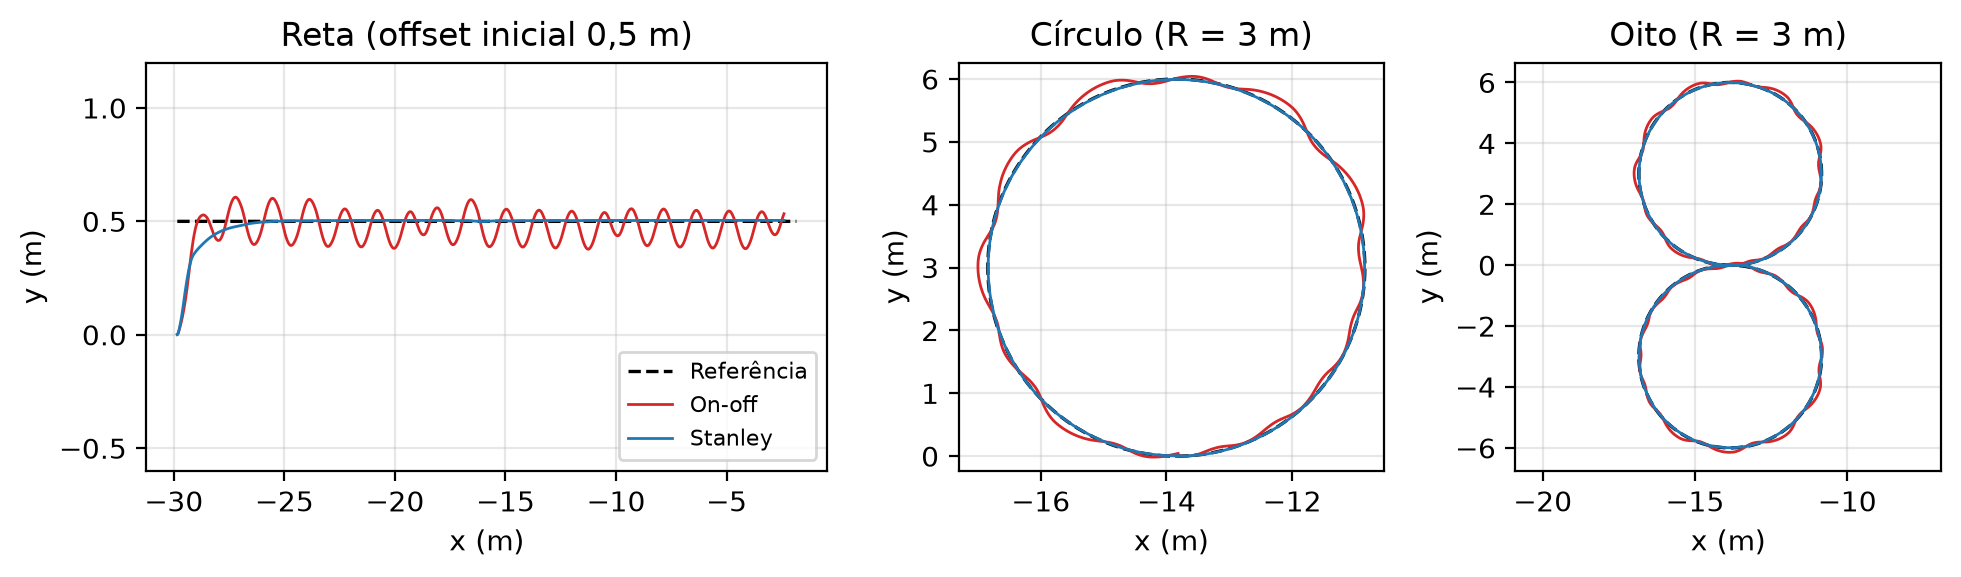
\includegraphics[width=\textwidth]{imgs/geo_trajetorias.png}
    \caption{Trajetória do eixo dianteiro com referências geométricas a $1{,}0\,\mathrm{m/s}$. Os erros são calculados com a pose verdadeira do simulador.}
    \label{fig:geo-trajetorias}
\end{figure}

\begin{table}[ht]
    \centering
    \caption{Erro lateral nas referências geométricas (após $5\,\mathrm{s}$): RMS e máximo, RMS da taxa de esterçamento e frequência de comutação do on-off.}
    \label{tab:geo}
    \small
    \setlength{\tabcolsep}{4pt}
    \begin{tabular}{llccccccc}
        \hline
        & & \multicolumn{4}{c}{On-off} & \multicolumn{3}{c}{Stanley} \\
        Referência & $v_{ref}$ & RMS & Máx. & $\dot\delta_{\mathrm{RMS}}$ & Comut. & RMS & Máx. & $\dot\delta_{\mathrm{RMS}}$ \\
        & $(\mathrm{m/s})$ & $(\mathrm{cm})$ & $(\mathrm{cm})$ & $(^\circ/\mathrm{s})$ & $(\mathrm{s^{-1}})$ & $(\mathrm{cm})$ & $(\mathrm{cm})$ & $(^\circ/\mathrm{s})$ \\
        \hline
        Reta    & $1{,}0$ & $6{,}5$  & $12{,}3$ & $48$ & $2{,}0$ & $0{,}37$ & $0{,}44$ & $11$ \\
                & $2{,}0$ & $28{,}2$ & $45{,}4$ & $43$ & $1{,}1$ & $0{,}20$ & $0{,}37$ & $15$ \\
        Círculo & $1{,}0$ & $8{,}3$  & $15{,}7$ & $48$ & $2{,}4$ & $0{,}45$ & $0{,}71$ & $4$ \\
                & $2{,}0$ & $36{,}4$ & $68{,}1$ & $44$ & $1{,}6$ & $0{,}39$ & $0{,}85$ & $3$ \\
        Oito    & $1{,}0$ & $7{,}7$  & $16{,}1$ & $48$ & $2{,}5$ & $0{,}47$ & $1{,}35$ & $5$ \\
                & $2{,}0$ & $38{,}1$ & $70{,}8$ & $43$ & $1{,}3$ & $0{,}73$ & $4{,}00$ & $7$ \\
        \hline
    \end{tabular}
\end{table}

O on-off mantém o veículo sobre as referências, mas em ciclo-limite: o esterçamento alterna continuamente e o erro oscila com amplitude de $12$--$16\,\mathrm{cm}$ a $1{,}0\,\mathrm{m/s}$. Ao dobrar a velocidade, o erro RMS aumenta de quatro a cinco vezes. O Stanley tem erro RMS abaixo de $1\,\mathrm{cm}$ em todos os casos e taxa de esterçamento de 3 a 15 vezes menor.

No oito (\autoref{fig:geo-oito}), o Stanley converge para $\approx5{,}7^\circ$, o valor de regime $\arctan(L/R)=5{,}75^\circ$, e o salto de curvatura no cruzamento ($t\approx19\,\mathrm{s}$) gera um pico de apenas $1{,}4\,\mathrm{cm}$. O on-off não tem esse nível e obtém a curvatura média alternando entre $+15^\circ$ e $0$ ou $-15^\circ$, o que gera a oscilação.

\begin{figure}[ht]
    \centering
    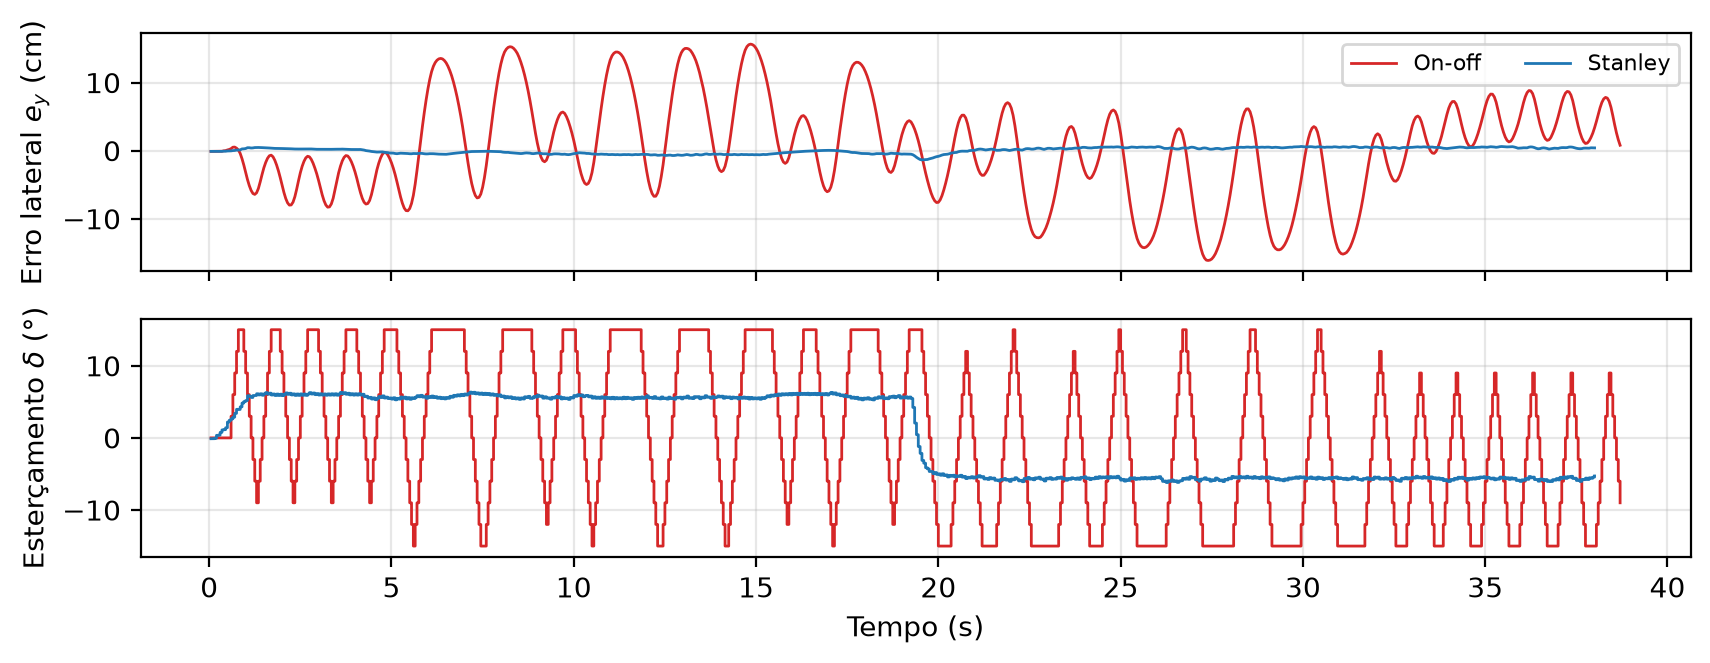
\includegraphics[width=\textwidth]{imgs/geo_oito_tempo.png}
    \caption{Erro lateral e esterçamento no oito a $1{,}0\,\mathrm{m/s}$. A troca de sentido da curva ocorre em $t\approx19\,\mathrm{s}$.}
    \label{fig:geo-oito}
\end{figure}

\textbf{Sensibilidade.} No on-off, o ciclo-limite cresce com a amplitude: no oito, o erro RMS foi de $4{,}1$, $7{,}7$ e $15{,}4\,\mathrm{cm}$ para $\delta_{on}=8$, $15$ e $20^\circ$. O valor de $8^\circ$ basta no oito, que exige $5{,}7^\circ$, mas não nas curvas mais fechadas da pista (\autoref{sec:res-visao}). No Stanley, partindo de $0{,}5\,\mathrm{m}$ de erro na reta, $k=0{,}5\,\mathrm{s^{-1}}$ converge lentamente (constante de tempo $\approx2{,}6\,\mathrm{s}$), $k=1{,}5\,\mathrm{s^{-1}}$ converge em $\approx4\,\mathrm{s}$ sem sobressinal e $k=5\,\mathrm{s^{-1}}$ apresenta sobressinal de $21\,\mathrm{cm}$, causado pela saturação em $20^\circ$ e pelo limite de taxa, ausentes da análise linearizada. Foi mantido $k=1{,}5\,\mathrm{s^{-1}}$.

\subsection{Seguimento da linha amarela pela câmera}\label{sec:res-visao}

A \autoref{fig:visao-pipeline} ilustra a cadeia de visão numa curva: os pontos projetados ficam a mais de $0{,}5\,\mathrm{m}$ do eixo dianteiro, e o ajuste local é extrapolado até ele. Nas voltas, a curvatura estimada teve percentil 99 de $\approx0{,}7\,\mathrm{m^{-1}}$ (raio de $1{,}4\,\mathrm{m}$), que exige $\approx12^\circ$ de esterçamento de regime.

\begin{figure}[ht]
    \centering
    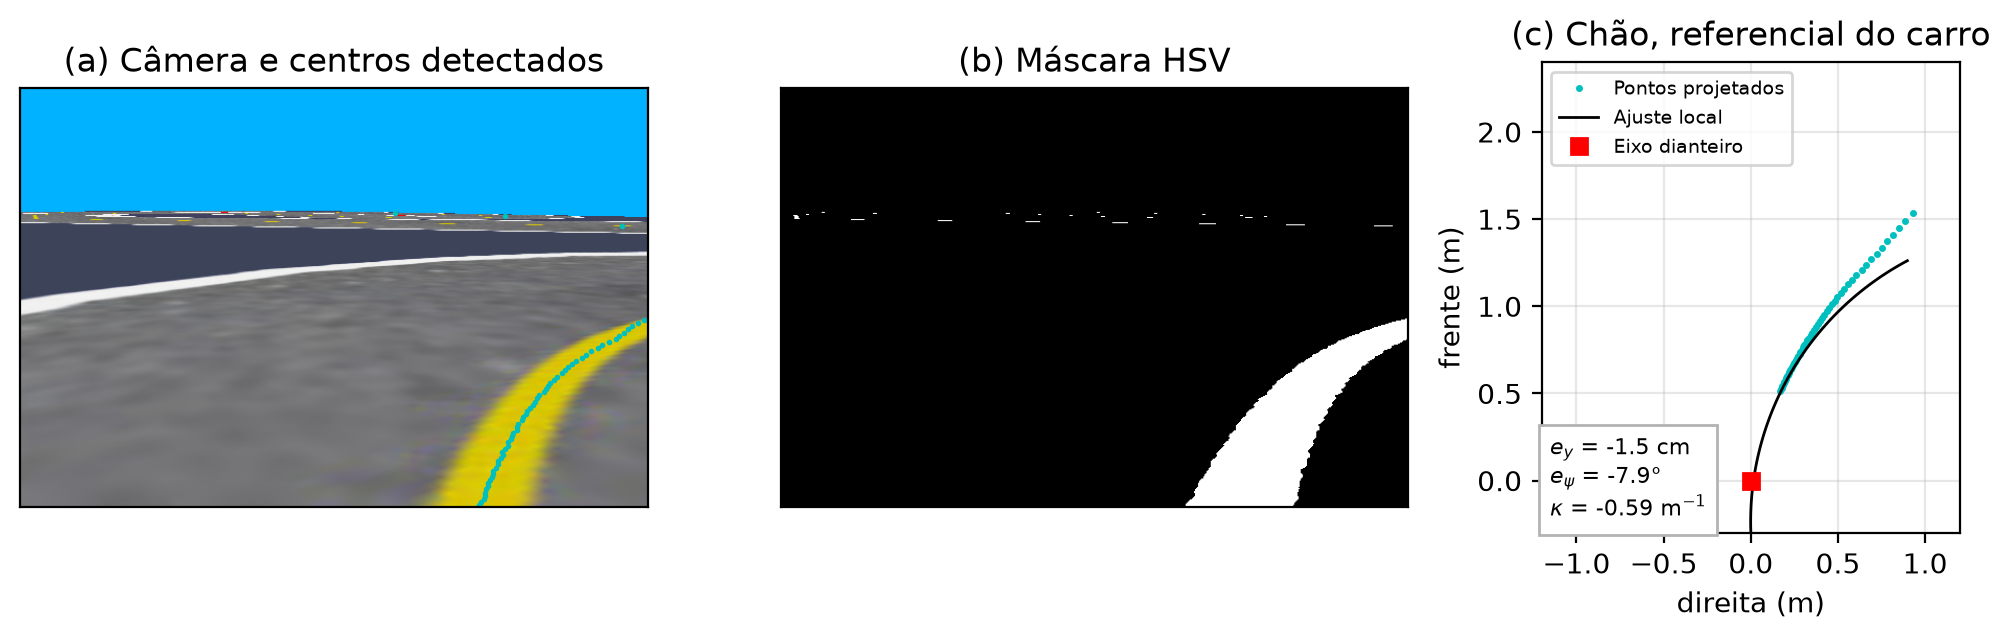
\includegraphics[width=\textwidth]{imgs/visao_pipeline.png}
    \caption{Cadeia de visão em um único quadro (sem memória): (a) imagem da câmera e centros da linha; (b) máscara HSV; (c) pontos projetados no chão, ajuste local e erros resultantes.}
    \label{fig:visao-pipeline}
\end{figure}

A \autoref{tab:visao} resume as voltas ($\approx246\,\mathrm{m}$) com velocidade constante. O Stanley completou o percurso em todas as velocidades, inclusive na máxima do veículo, $2{,}5\,\mathrm{m/s}$, em $99{,}7\,\mathrm{s}$. O on-off só completou a volta a $0{,}5$ e $0{,}75\,\mathrm{m/s}$; a partir de $1{,}0\,\mathrm{m/s}$ falhou cada vez mais cedo.

\begin{table}[ht]
    \centering
    \caption{Volta completa com referência visual e $v_{ref}$ constante. Erros verdadeiros medidos em relação à linha da textura, após $5\,\mathrm{s}$; a última coluna é o RMS do erro estimado pela câmera.}
    \label{tab:visao}
    \small
    \setlength{\tabcolsep}{3.5pt}
    \begin{tabular}{llcccccc}
        \hline
        Controlador & $v_{ref}$ & Resultado & Tempo & RMS & P95 & Máx. & RMS visual \\
        & $(\mathrm{m/s})$ & & $(\mathrm{s})$ & $(\mathrm{cm})$ & $(\mathrm{cm})$ & $(\mathrm{cm})$ & $(\mathrm{cm})$ \\
        \hline
        On-off  & $0{,}5$  & volta completa & $488{,}9$ & $2{,}8$ & $6{,}0$ & $10{,}6$ & $3{,}1$ \\
                & $0{,}75$ & volta completa & $328{,}3$ & $3{,}4$ & $6{,}3$ & $10{,}4$ & $3{,}9$ \\
                & $1{,}0$  & perdeu a linha ($163\,\mathrm{m}$) & $161{,}2$ & $7{,}0$ & $12{,}3$ & $48{,}5$ & $6{,}9$ \\
                & $1{,}5$  & perdeu a linha ($91\,\mathrm{m}$) & $60{,}7$ & $12{,}8$ & $21{,}9$ & $52{,}9$ & $12{,}0$ \\
                & $2{,}0$  & saiu da pista ($53\,\mathrm{m}$) & $27{,}1$ & $26{,}1$ & $42{,}3$ & $101$ & $23{,}3$ \\
                & $2{,}5$  & saiu da pista ($21\,\mathrm{m}$) & $9{,}7$ & $54{,}0$ & $86{,}6$ & $104$ & $44{,}9$ \\
        \hline
        Stanley & $1{,}0$ & volta completa & $245{,}6$ & $1{,}0$ & $2{,}3$ & $5{,}7$ & $0{,}6$ \\
                & $1{,}5$ & volta completa & $164{,}3$ & $1{,}1$ & $2{,}2$ & $6{,}1$ & $0{,}9$ \\
                & $2{,}0$ & volta completa & $123{,}8$ & $1{,}7$ & $3{,}3$ & $16{,}9$ & $1{,}8$ \\
                & $2{,}5$ & volta completa & $99{,}7$ & $3{,}6$ & $4{,}9$ & $33{,}0$ & $3{,}8$ \\
        \hline
    \end{tabular}
\end{table}

A \autoref{fig:pista} compara os controladores a $1{,}0\,\mathrm{m/s}$. O on-off oscila durante todo o percurso e perde a linha no canto mais fechado, em $(-1{,}5;\ 9{,}4)\,\mathrm{m}$: o comando estava em $-15^\circ$ quando a linha começou a curvar para a esquerda, o erro de orientação chegou a $33^\circ$, acima da meia abertura da câmera ($30^\circ$), e a linha saiu da imagem. Em velocidades maiores a falha ocorre antes; a $2{,}5\,\mathrm{m/s}$, ainda na reta inicial. O Stanley mantém o erro abaixo de $2{,}3\,\mathrm{cm}$ em $95\%$ da volta; os maiores erros ocorrem nos dois cantos vivos da linha.

\begin{figure}[ht]
    \centering
    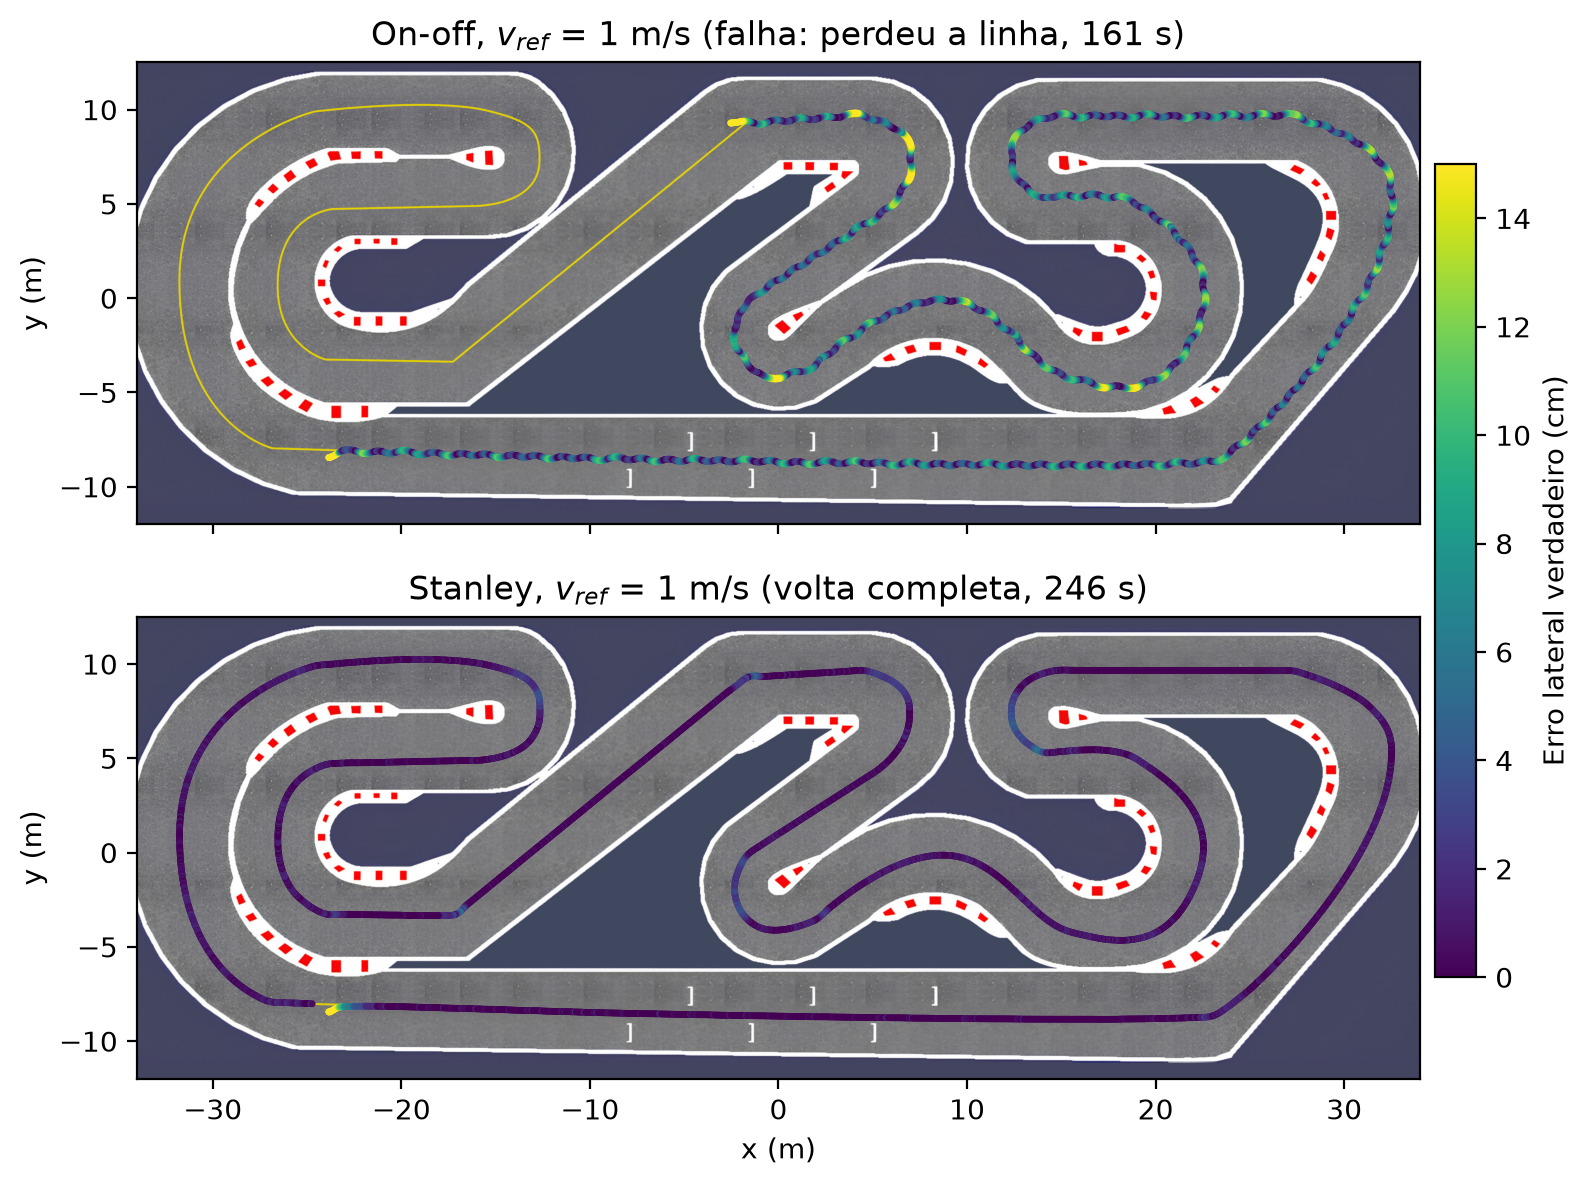
\includegraphics[width=0.88\textwidth]{imgs/pista_1.png}
    \caption{Trajetória do eixo dianteiro sobre a pista a $1{,}0\,\mathrm{m/s}$, colorida pelo erro lateral verdadeiro. O carrinho parte de $(-24;\ -8{,}5)\,\mathrm{m}$ e percorre a pista no sentido anti-horário.}
    \label{fig:pista}
\end{figure}

Com a velocidade, o erro do Stanley cresce sobretudo nesses cantos: a $2{,}5\,\mathrm{m/s}$ o pico foi de $33\,\mathrm{cm}$, com RMS de $3{,}6\,\mathrm{cm}$ e inclinação máxima da carroceria de $9{,}3^\circ$, longe do capotamento. A linha foi detectada em $100\%$ dos passos, e o RMS estimado pela câmera ficou próximo do verdadeiro, indicando que a visão não introduz viés significativo.

\textbf{Redução nas curvas.} Com $v_{ref}=2{,}5\,\mathrm{m/s}$ e redução nas curvas, o Stanley completou a volta em $107{,}9\,\mathrm{s}$ (média de $2{,}28\,\mathrm{m/s}$), só $8\%$ a mais, enquanto o erro RMS caiu de $3{,}6$ para $1{,}8\,\mathrm{cm}$, o pico de $33{,}0$ para $17{,}4\,\mathrm{cm}$ e a inclinação de $9{,}3^\circ$ para $2{,}9^\circ$. O on-off, nas mesmas condições, perdeu a linha após $52\,\mathrm{m}$, pois a oscilação nas retas, em velocidade máxima, já é excessiva.

\textbf{Amplitude do on-off na pista.} Com $\delta_{on}=8^\circ$, o veículo completou a volta a $0{,}5\,\mathrm{m/s}$, mas com pico de $23{,}4\,\mathrm{cm}$ (contra $10{,}6\,\mathrm{cm}$ com $15^\circ$), e a $0{,}75\,\mathrm{m/s}$ perdeu a linha após $178\,\mathrm{m}$, numa curva com curvatura estimada de $1{,}2\,\mathrm{m^{-1}}$. Com $8^\circ$ o menor raio possível é $L/\tan8^\circ=2{,}1\,\mathrm{m}$, o que confirma a escolha de $15^\circ$.

\subsection{Validação no veículo real}\label{sec:res-real}

O Stanley foi testado no carrinho físico, seguindo uma fita amarela no piso de um corredor, com a mesma lei e os mesmos parâmetros do simulador. A faixa é detectada em HSV numa imagem de $320\times240$ pixels e convertida para o chão por uma homografia calibrada com pontos medidos a partir do eixo dianteiro. O controle longitudinal é o PI do veículo real desenvolvido na Parte 1 ($k_p=1$, $k_i=0{,}8$ e \textit{feedforward}). Foram realizados sete ensaios de $30\,\mathrm{s}$; o on-off não foi testado no veículo real.

\begin{table}[ht]
    \centering
    \caption{Ensaios do Stanley no carrinho real. Os erros são estimados pela câmera (não há referência independente) e calculados somente com a faixa detectada.}
    \label{tab:real}
    \small
    \setlength{\tabcolsep}{3.5pt}
    \begin{tabular}{ccccccl}
        \hline
        Ensaio & $v_{ref}$ & Faixa & RMS $e_y$ & Máx. $|e_y|$ & RMS $e_\psi$ & Término \\
        & $(\mathrm{m/s})$ & detectada & $(\mathrm{cm})$ & $(\mathrm{cm})$ & $(^\circ)$ & \\
        \hline
        1 & $0{,}63$ & $99{,}4\%$ & $2{,}1$ & $16{,}3$ & $5{,}4$ & $30\,\mathrm{s}$ completos \\
        2 & $0{,}63$ & $100\%$ & $2{,}6$ & $15{,}9$ & $7{,}7$ & parada por obstáculo ($22\,\mathrm{s}$) \\
        3 & $0{,}63$ & $100\%$ & $2{,}0$ & $4{,}6$ & $5{,}7$ & falha de leitura do encoder ($21\,\mathrm{s}$) \\
        4 & $1{,}29$ & $100\%$ & $5{,}3$ & $9{,}7$ & $5{,}1$ & parada por obstáculo ($8\,\mathrm{s}$) \\
        5 & $0{,}61$ & $71{,}3\%$ & $5{,}3$ & $31{,}0$ & $14{,}2$ & perdas da faixa a partir de $8{,}6\,\mathrm{s}$ \\
        6 & $0{,}63$ & $95{,}5\%$ & $2{,}9$ & $21{,}0$ & $5{,}7$ & $30\,\mathrm{s}$ completos \\
        7 & $0{,}63$ & $99{,}0\%$ & $2{,}6$ & $4{,}8$ & $4{,}7$ & $30\,\mathrm{s}$ completos \\
        \hline
    \end{tabular}
\end{table}

A \autoref{tab:real} resume os ensaios e a \autoref{fig:real} mostra o ensaio 7. Nos ensaios sem interrupções (1, 6 e 7), o RMS do erro estimado ficou entre $2{,}1$ e $2{,}9\,\mathrm{cm}$, da mesma ordem do simulador, e a velocidade acompanhou a referência de $\approx0{,}63\,\mathrm{m/s}$. No ensaio 4, a $1{,}29\,\mathrm{m/s}$, a faixa foi mantida por $8\,\mathrm{s}$ até a parada pelo ultrassom. No ensaio 5, a faixa não foi detectada em $29\%$ das amostras.

Exceto no ensaio 5, os erros médios foram positivos ($e_y\approx+1{,}4$ a $+4{,}4\,\mathrm{cm}$, $e_\psi\approx+3$ a $+5^\circ$) e o esterçamento médio ficou em $6$--$7^\circ$, embora a curvatura estimada da faixa fosse próxima de zero. A informação visual chegou ao controle com idade mediana de $\approx0{,}15\,\mathrm{s}$.

\begin{figure}[ht]
    \centering
    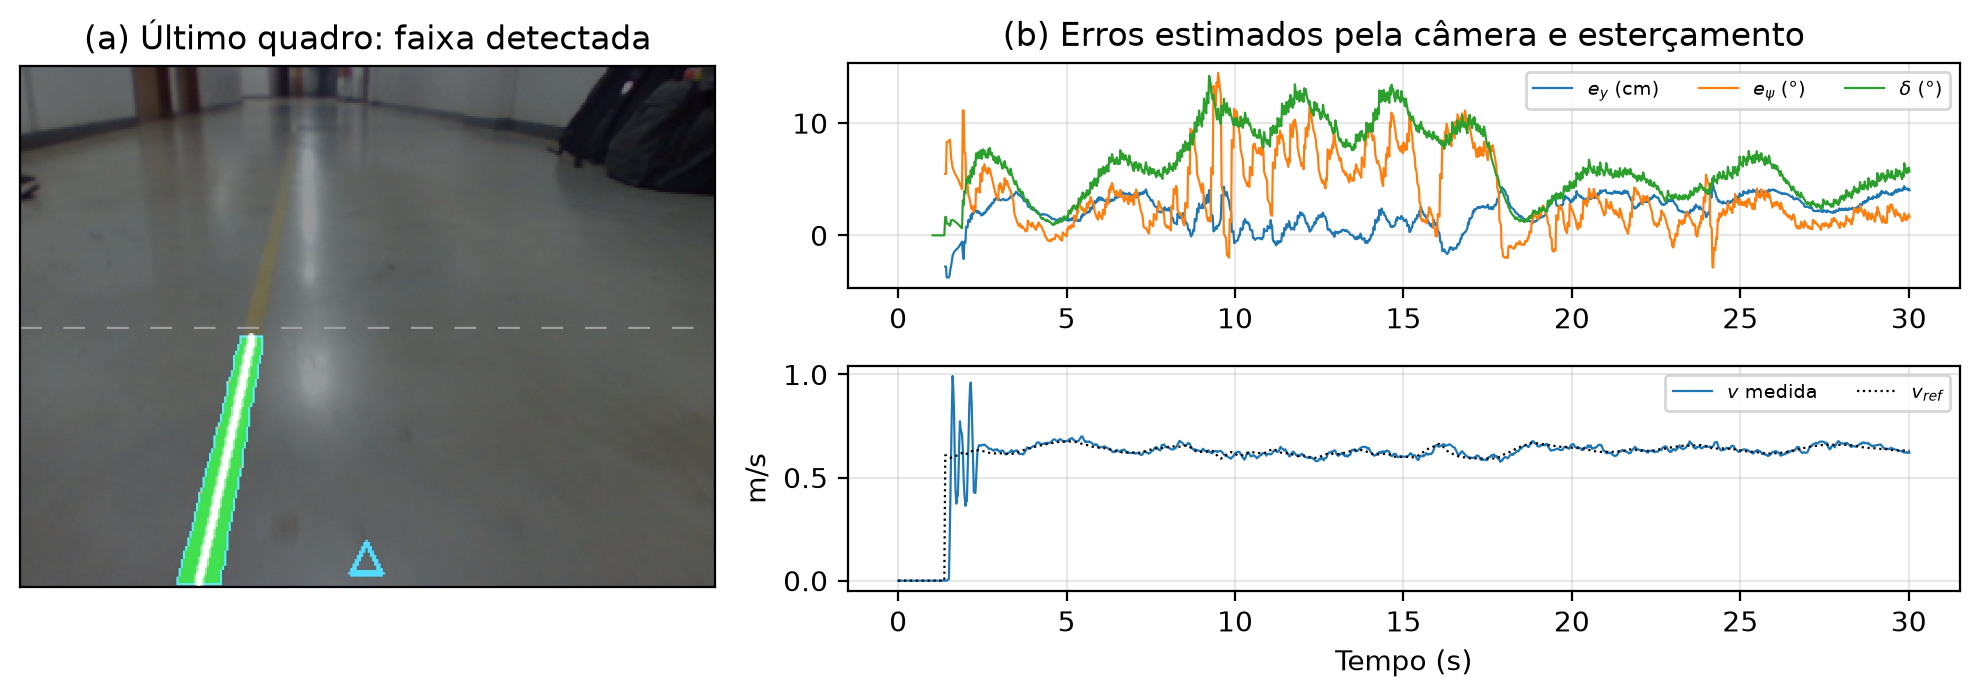
\includegraphics[width=0.92\textwidth]{imgs/real_stanley.png}
    \caption{Ensaio 7 do Stanley no carrinho real: (a) último quadro, com a faixa detectada em verde; (b) erros estimados pela câmera, esterçamento, velocidade e referência.}
    \label{fig:real}
\end{figure}
